%%%%%%%%%%%%%%%%%%%%%%%%%%%%%%%%%%%%%%%%%%%%%%%%%%%%%%%%%%%%
%% Chapter 4 - Data Generation and Preparation (10-16 pages)
%% Purpose: explain how the Simscape datasets were designed to
%% contain realistic operation, causal actuator excitation, and
%% variation required for robust and adaptive learning.
%%%%%%%%%%%%%%%%%%%%%%%%%%%%%%%%%%%%%%%%%%%%%%%%%%%%%%%%%%%%
\chapter{Data Generation and Preparation}
\label{chap:data}

Chapter~\ref{chap:system} defined two plant representations: detailed
hydraulics in Simscape and fast rigid-body dynamics in IsaacLab. This chapter
documents the datasets that connect them, including collection, auditing,
feature construction and splitting. Table~\ref{tab:sys:provenance} records
their provenance.

\emph{Simscape campaigns.} Closed-loop runs provide realistic operating data
for the inverse and reduced-order models. Separate open-loop valve excitation
provides the causal command information needed by the strict forward model
(Section~\ref{sec:data:open-loop}).

\emph{ROM calibration.} After Simscape training, the command ROM was
fine-tuned on five closed-loop IsaacLab reference shapes. Only its bounded
correction head remained trainable, with Simscape replay retained
(Section~\ref{sec:data:rom-calibration}). The ID--FD pair was not calibrated
in IsaacLab.

\emph{IsaacLab deployment data.} The system-dynamics surrogate, the privileged
encoder and the adaptation module use two $118$-run collections recorded in the
deployed command
ROM--PhysX plant, including dedicated PRBS windows
(Section~\ref{sec:data:isaaclab}). No earlier adaptation or system-dynamics
model was reused. Figure~\ref{fig:data:pipeline} summarises the common
preparation workflow.

\begin{figure}[p]
  \centering
  \begin{tikzpicture}[x=1cm,y=1cm,>=Latex,font=\small,
    source/.style={draw=black!55,line width=.8pt,rounded corners=2pt,
      fill=white,minimum width=3.05cm,minimum height=1.25cm,
      align=center,inner sep=3pt},
    process/.style={draw=black!55,line width=.8pt,rounded corners=2pt,
      fill=white,minimum width=5.4cm,minimum height=1.08cm,
      align=center,font=\small},
    output/.style={draw=black!65,line width=.8pt,rounded corners=2pt,
      fill=white,minimum width=3.05cm,minimum height=1.35cm,
      align=center,font=\small},
    stage/.style={circle,draw=black!70,fill=white,text=black,
      line width=.8pt,minimum size=7mm,inner sep=0pt,font=\small\bfseries},
    flow/.style={-{Latex[length=2.2mm]},line width=.8pt,draw=black!75},
    bus/.style={line width=.8pt,draw=black!65}]

    \node[font=\large\bfseries,text=black!80] at (0,.65) {DATA COLLECTION};
    \draw[black!40] (-6.95,.25) -- (6.95,.25);
    \node[font=\small\bfseries,text=black!80] at (-3.50,-.12) {SIMSCAPE};
    \node[font=\small\bfseries,text=black!80] at (3.50,-.12)
      {ISAACLAB / DEPLOYMENT};
    \node[draw=black!60,line width=.7pt,rounded corners=5pt,
      fill=white,minimum width=6.25cm,minimum height=.48cm,
      font=\scriptsize,text=black!75] at (-3.50,-.67)
      {\textbf{Randomised campaign}\quad $1\,000$ runs $\cdot$ $12$ parameters};

    \node[source] (closed) at (-5.25,-1.85)
      {\textbf{Closed-loop}\\[-1pt]\footnotesize $1\,040$ runs};
    \node[source] (open) at (-1.75,-1.85)
      {\textbf{Open-loop}\\[-1pt]\footnotesize $4$ runs};
    \node[source] (romsrc) at (1.75,-1.85)
      {\textbf{ROM calibration}\\[-1pt]\footnotesize $5$ references};
    \node[source] (adapt) at (5.25,-1.85)
      {\textbf{Adaptation data}\\[-1pt]\footnotesize $118$ runs};
    \coordinate (collectbus) at (0,-2.85);
    \foreach \s in {closed,open,romsrc,adapt}{
      \draw[line width=.8pt,black!70] (\s.south) -- (\s.south |- collectbus);}
    \draw[line width=.8pt,black!70] (-5.25,-2.85) -- (5.25,-2.85);

    \node[process] (extract) at (0,-3.90)
      {\textbf{EXTRACT \& ALIGN}\\[-1pt]\footnotesize states $\bullet$ actions $\bullet$ targets};
    \node[stage] at (-3.25,-3.90) {1};
    \draw[flow] (collectbus) -- (extract.north);

    \node[diamond,aspect=2.15,draw=black!75,line width=.9pt,
      fill=black!12,align=center,inner sep=2pt,font=\footnotesize\bfseries]
      (audit) at (0,-5.90)
      {QUALITY AUDIT\\[-1pt]\scriptsize validity $\bullet$ excitation};
    \node[stage] at (-3.25,-5.90) {2};
    \draw[flow] (extract.south) -- (audit.north);

    \node[draw=rltred,line width=1.5pt,rounded corners=2pt,
      fill=rltred!10,minimum width=2.80cm,minimum height=1.10cm,
      align=center,font=\footnotesize\bfseries] (recollect) at (5.55,-5.90)
      {RECOLLECT\\[-1pt]OR REDESIGN};
    \draw[-{Latex[length=2.2mm]},line width=1.3pt,rltred]
      (audit.east) -- (recollect.west);
    \node[anchor=south,fill=white,inner sep=1pt,
      font=\scriptsize\bfseries,text=rltred]
      at ($(audit.east)!.50!(recollect.west)+(0,1.7mm)$) {FAIL};
    \draw[-{Latex[length=2.0mm]},line width=1.0pt,dashed,rltred]
      (recollect.east) |- (5.25,-2.85);

    \node[process,draw=rltgreen,fill=rltgreen!10,line width=1.5pt]
      (split) at (0,-8.20)
      {\textbf{SPLIT BY RUN}\\[-1pt]\footnotesize train $\bullet$ validation $\bullet$ test};
    \node[stage] at (-3.25,-8.20) {3};
    \draw[-{Latex[length=2.2mm]},line width=1.3pt,rltgreen]
      (audit.south) -- (split.north);
    \node[anchor=west,fill=white,inner sep=1pt,
      font=\scriptsize\bfseries,text=rltgreen]
      at ($(audit.south)!.38!(split.north)+(4.0mm,0)$) {PASS};

    \node[process] (normalise) at (0,-10.20)
      {\textbf{NORMALIZE}\\[-1pt]\footnotesize training statistics only};
    \node[stage] at (-3.25,-10.20) {4};
    \draw[flow] (split.south) -- (normalise.north);

    \coordinate (outbus) at (0,-12.50);
    \draw[bus] (normalise.south) -- (0,-11.27);
    \draw[bus] (0,-12.02) -- (outbus);
    \draw[line width=.8pt,black!65] (-5.25,-12.50) -- (5.25,-12.50);
    \node[font=\large\bfseries,text=black!80,fill=white,inner sep=2pt]
      at (0,-11.65) {MODEL DATASETS};
    \draw[black!40] (-6.95,-12.02) -- (-2.55,-12.02);
    \draw[black!40] (2.55,-12.02) -- (6.95,-12.02);

    \node[output] (inverse) at (-5.25,-13.55)
      {\textbf{Inverse model}\\[-1pt]\footnotesize closed-loop data};
    \node[output] (forward) at (-1.75,-13.55)
      {\textbf{Forward model}\\[-1pt]\footnotesize open-loop data};
    \node[output] (romout) at (1.75,-13.55)
      {\textbf{ROM}\\[-1pt]\footnotesize calibrated dynamics};
    \node[output] (aamout) at (5.25,-13.55)
      {\textbf{AAM}\\[-1pt]\footnotesize adaptation history};
    \foreach \o in {inverse,forward,romout,aamout}{
      \draw[-{Latex[length=2.2mm]},line width=.8pt,black!70]
        (\o.north |- outbus) -- (\o.north);}
  \end{tikzpicture}
  \caption{Data-preparation workflow. Two Simscape collections and two
  IsaacLab collections pass through common extraction, audit, run-level
  splitting and training-statistics normalisation stages. The randomised
  Simscape campaign is provenance metadata rather than a pipeline stage. A
  failed audit returns the experiment to collection; accepted material forms
  the inverse, forward, ROM and AAM datasets.}
  \label{fig:data:pipeline}
\end{figure}

\section{Dataset Objectives and Design Requirements}
\label{sec:data:objectives}



Four requirements governed collection and preparation.

\begin{description}
  \item[R1: realistic operating distribution.] The learned models are
    deployed inside a tracking controller, so they must be accurate in the
    states that controller visits, namely coordinated multi-axis motion,
    gravity-loaded poses and moderate speeds.
  \item[R2: causal identifiability of the valve.] A forward model is
    only useful to a policy if it responds to the command. This requires
    that the valve signal in the training data carry information that the
    state history does not already carry, which is a property of the
    \emph{experiment}, not of the network~\cite{ljung1999system,
    isermann2011identification}.
  \item[R3: variation across a plant family.] Robust training and online
    adaptation both need many plants rather than one. The variation must be
    physically meaningful, must demonstrably change the measured response, and
    must be recorded per run, because the privileged plant context of
    Section~\ref{sec:data:system-dynamics} is computed from those factors.
  \item[R4: clean separation.] Train, validation and test material must be
    separable at the level of complete runs, so that no transition window
    straddles a split boundary and no run contributes to two splits.
\end{description}

R1 and R2 require different experiments. Closed-loop control gives realistic
motion but correlates command with state; open-loop excitation breaks that
correlation but is less representative of deployment. The two campaigns are
therefore retained and combined as described in
Section~\ref{sec:data:combining}.

\section{Randomised Parameter Space of the Simscape Campaign}
\label{sec:data:randomization}

This section records the Simscape randomisation design as collection provenance.
No reported model is trained on this curriculum. The export the actuator models
are actually fitted on is a separate closed-loop collection on the nominal
plant (Section~\ref{sec:data:combining}). The curriculum is kept because its
compliance analysis informed the IsaacLab factor design of
Section~\ref{sec:data:factors}.

Plants are drawn from a twelve-dimensional space by Latin hypercube
sampling~\cite{mckay1979comparison}, fixed once before any simulation runs, so
the parameter table can be audited independently of the data it produced. The
batch is a curriculum rather than a homogeneous pool: run~1 is the nominal
plant, runs 2--251 randomise only the hydraulics, runs 252--501 only the
mechanics, and runs 502--1000 both (Figure~\ref{fig:data:design}(a)), so a
modelling failure can be attributed to one axis by retraining on one block.
Appendix~\ref{app:dataset} lists the axes and
Appendix~\ref{app:data:curriculum} the generation procedure.

\begin{figure}[tb]
  \centering
  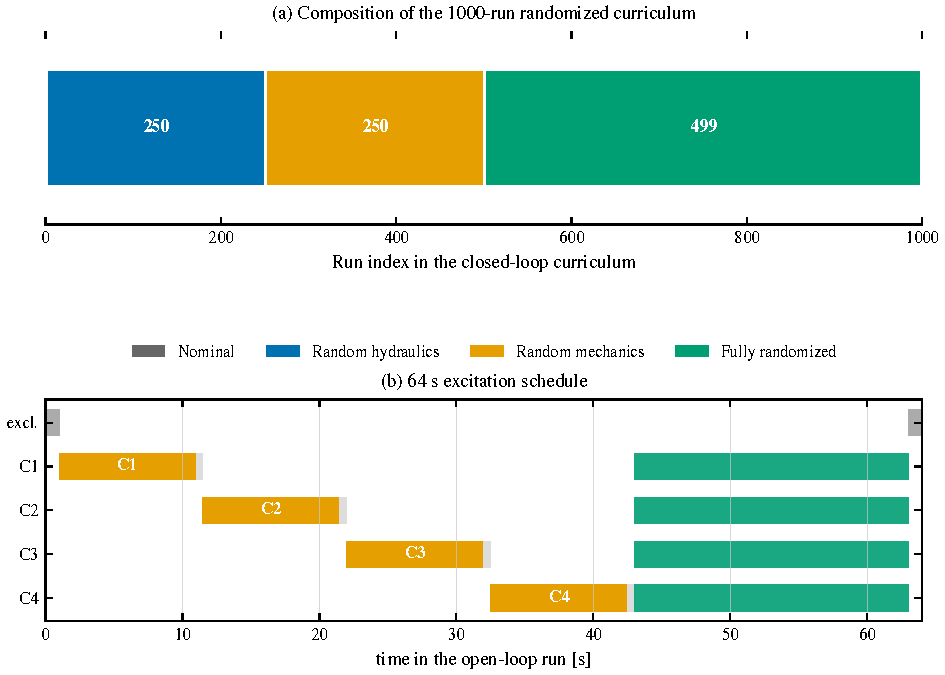
\includegraphics[width=\textwidth]{images/ch4/ch4_dataset_design}
  \caption{Design of the two collection campaigns.
  (a)~Composition of the closed-loop curriculum: one nominal run, then $250$
  hydraulics-only, $250$ mechanics-only and $499$ fully randomised draws.
  (b)~Timeline of one open-loop excitation run.}
  \label{fig:data:design}
\end{figure}

Two design choices carry into the deployment factors. Seal wear is one sampled
number driving three parameters together, so a worn cylinder becomes leakier and
slower at once: it scales piston clearance linearly, valve leakage area with the
cube of the same factor, and the spool time constant from $\unit[8]{ms}$ to
about $\unit[13]{ms}$ at the top of the range. Sampling the three independently
would have produced machines that are very leaky and yet perfectly fast. The
entrained-air and dead-volume coordinates randomise chamber dead volume over
$505$ to $\unit[579]{mL}$, which reaches the pressure dynamics through the
chamber volume in Equation~\eqref{eq:sys:continuity}, so compressibility enters
the batch as capacitance variation. The mechanical axes perturb all fourteen
rigid bodies: mass by up to $\pm 20\,\%$, centre of mass by up to $\pm 5\,\%$
of its nominal offset, and the inertia tensor consistently with the mass change,
so each body remains physically realisable. Joint stiffness and damping model
compliance in the bearings and linkage rather than in the fluid, and set how
much of a pressure transient appears as boom oscillation instead of clean
motion.

\section{Closed-Loop Data Collection}
\label{sec:data:closed-loop}

Algorithm~\ref{alg:data:closed-loop} in Appendix~\ref{app:data:curriculum}
gives the procedure that produced the curriculum above. The parameter table is
fixed before simulation and each run receives a new reference path.

\subsection{The Controller as a Data-Collection Instrument}

Every closed-loop run uses the same integral-backstepping controller at
$\unit[0.005]{s}$. Its gains remain fixed, so response differences are caused
by the plant draw rather than controller retuning.

Joint~2 uses PI control with velocity damping and gravity bias because it
carries the boom load. A barrier term enforces the URDF limits. Per-axis
command limits are $[0.95,\,0.95,\,0.80,\,0.80,\,0.90]$; the first four are
also stored in the inverse-dynamics checkpoint
(Section~\ref{sec:models:id}).

\section{Open-Loop Excitation Experiments}
\label{sec:data:open-loop}

\subsection{Limitations of the Closed-Loop Batch}

The first forward model achieved one-step $R^2\approx0.999$ on closed-loop
data but was almost insensitive to valve input: zeroing the input changed
long-horizon error by only a few percent
(Section~\ref{sec:models:fd-identifiability}). In closed loop, command is
largely determined by the state history already given to the model, so the
data do not separate command causality from state correlation
~\cite{ljung1999system}.

Figure~\ref{fig:data:regimes} confirms that coverage alone is not the issue.
The valve is saturated for about one quarter of a pooled run, operates at
mid-authority for roughly half, and otherwise remains in low-command creep.
Despite this spread, command and cylinder velocity remain concentrated along a
narrow band. The data are diverse in control effort but not identifiable,
motivating a separate open-loop experiment.

\begin{figure}[tb]
  \centering
  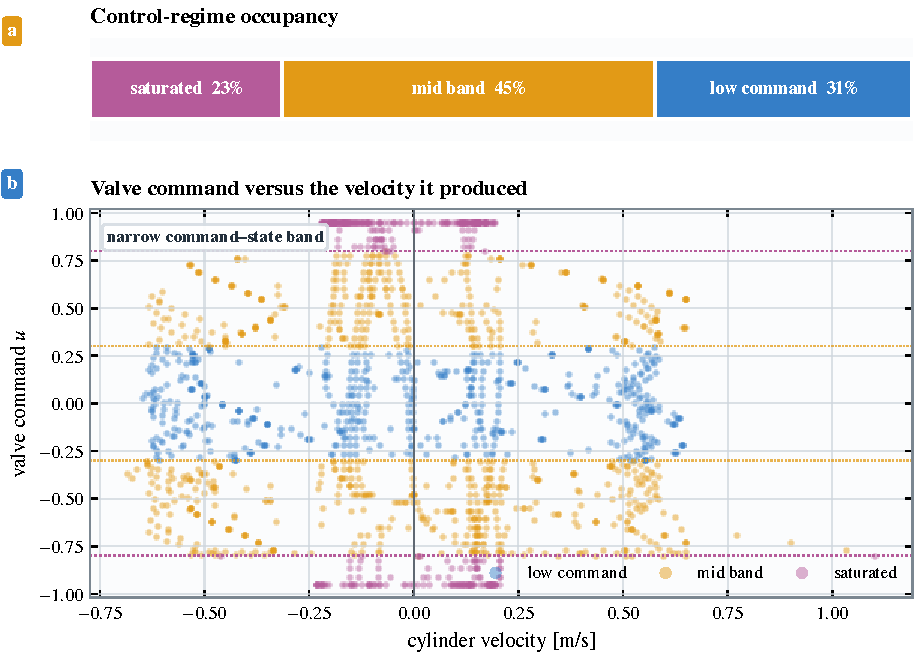
\includegraphics[width=\textwidth]{images/ch4/ch4_regimes}
  \caption{The closed-loop batch is diverse in control effort but
  not identifiable. (a)~Fraction of time the valve spends saturated, in the mid
  band and in low-command creep. (b)~The same run in the command--state plane,
  where the correlation that blocks identification is visible.}
  \label{fig:data:regimes}
\end{figure}

\subsection{Design of the Excitation Signal}

The excitation run lasts $\unit[64]{s}$ and follows the fixed schedule in
Figure~\ref{fig:data:design}(b). One second of startup is discarded, because
those samples describe the initialisation rather than the dynamics. Four
sequential slots follow, each giving one cylinder ten seconds of excitation
followed by a half-second zero-command gap that makes the segment boundaries
unambiguous. A twenty-second phase then drives all four channels at once, and a
final second of zero command closes the run. Commands are limited to $\pm 0.90$
of full authority.

An initial rapidly switching signal met the formal persistence condition but
kept each piston near one stroke position. The final design instead uses long
full-authority plateaus in the sequential phase and slow, high-authority motion
in the simultaneous phase. A slow near-square cycle is combined with distinct
medium-frequency channel components, with raised-cosine entry and exit ramps.
This provides both input excitation and useful stroke coverage.

\subsection{Plant Draws and Acceptance}

The same excitation is applied to four plant draws from the parameter space of
the closed-loop campaign: nominal, randomised hydraulics, randomised mechanics
and fully randomised. Holding the input fixed and varying only the plant makes
the four runs directly comparable.

Each run is checked for stroke coverage before acceptance, the collector
requiring at least $10\,\%$ of available stroke on cylinders 1--3 and $8\,\%$ on
cylinder 4. The retained runs cover $33\,\%$ of the stroke on cylinder 1 and
$12\,\%$ on cylinder 4, the narrowest of the four. Every channel clears the
floor, and Section~\ref{sec:data:diagnostics} confirms the material is
informative at these coverages.

The acceptance checks in Section~\ref{sec:data:diagnostics} verify that every
export contains independent state trajectories.

\section{Combining Closed-Loop and Open-Loop Datasets}
\label{sec:data:combining}

The inverse model uses only closed-loop data because its target is the
controller command for a measured state. The forward model is retrained on the
strict open-loop export while retaining closed-loop replay at weight $0.25$.
Without replay, four excitation runs do not provide enough pose coverage.

Figure~\ref{fig:data:coverage} shows the difference: closed-loop data covers
the reachable range, while open-loop data concentrates at identifiable valve
plateaus. The forward model therefore uses both.

\begin{figure}[tb]
  \centering
  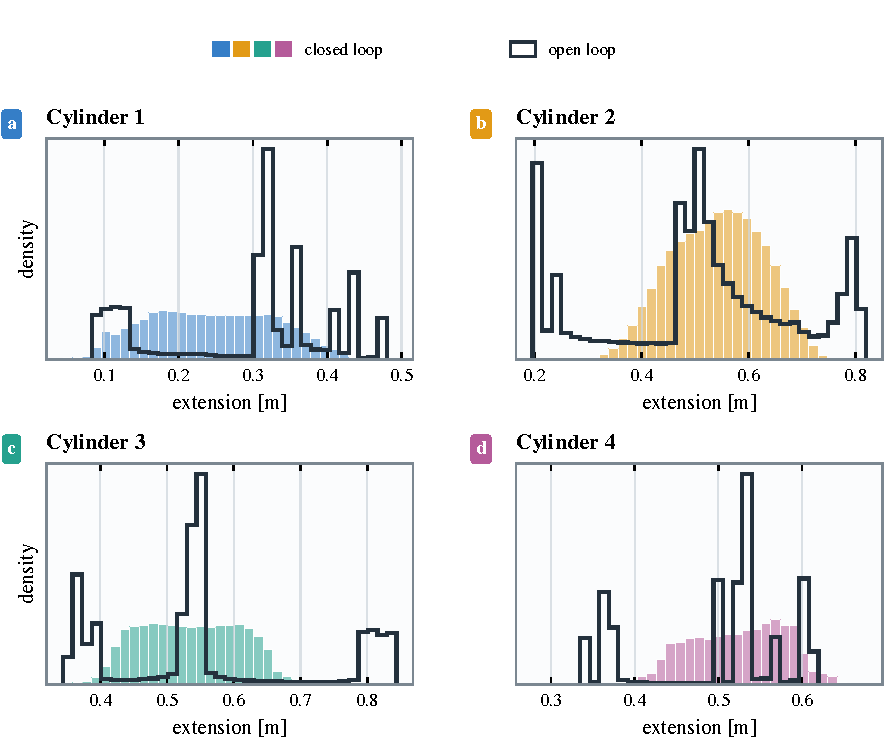
\includegraphics[width=\textwidth]{images/ch4/ch4_coverage}
  \caption{Extension coverage of the two campaigns, per cylinder
  and pooled over runs (closed-loop filled, open-loop outline). The closed-loop
  data fills the reachable range smoothly; the open-loop data concentrates into
  the plateaus where the valve is identifiable.}
  \label{fig:data:coverage}
\end{figure}

For ROM training, the inverse and forward exports are joined by run identifier,
time index and sample time. The join is accepted only when their
sixteen-dimensional cylinder states match sample for sample. It contains
$452\,400$ transitions at $\unit[0.05]{s}$ from $1\,040$ runs, split into
$936$/$52$/$52$ complete runs. Valve command is used only to supervise the
ROM's internal valve head; it is not a runtime input
(Section~\ref{sec:models:rom}).

This aligned nominal-plant export trains the inverse, forward and ROM models and
ships with the project, so every model-level result can be recomputed from the
file that produced it. Exact alignment, increment consistency and the
identifiability failure were checked directly on that export.


\section{Closed-Loop Calibration Data for the Command ROM}
\label{sec:data:rom-calibration}

The ROM drives a PhysX articulation whose compliance and contact response are
not present in Simscape. Further Simscape training cannot remove the resulting
deployment offset.

The calibration set therefore comes from closed-loop ROM--PhysX operation on
the native $\unit[0.05]{s}$ grid. Its $4\,084$ transitions store the six-step
runtime history and measured PhysX transition.

Only the command-gated correction head is trainable; all other parameters are
frozen and the correction is capped at $\unit[3]{mm}$. Original-data replay at
weight $0.25$ preserves wider pose coverage. The gate makes the correction
zero at zero command, retaining stationary hold.

The trajectories predate the moving-verge benchmark and exclude
cutter--ground contact. The bounded head limits, but does not remove, this
coverage gap. Section~\ref{sec:sys:rom-is-plant} explains the consequence for
the three-way comparison.

\section{The IsaacLab Deployment Collections}
\label{sec:data:isaaclab}

Two collections are recorded in the deployment plant. They share their factor
design, their domains, their splits and their freezing procedure, and differ in
one respect only: how the arm is driven. The first is driven by the task
controller and is the collection the inverse and forward models are scored
against in Section~\ref{sec:models:id-trust}; the second is driven by open-loop
excitation and is the one the adaptation module is trained on. Why both exist is
itself a result, and it is given in
Section~\ref{sec:data:openloop-collection}.

\subsection{Provenance of the Deployment Data}

The models that carry the identifiability argument, namely the system-dynamics
surrogate, the privileged factor encoder and the offline history encoder,
describe the plant the adaptive controller is closed around. That plant is the
command ROM plus PhysX, not the Simscape model. A surrogate identified on
Simscape data would be a model of a model, and the latent it defines would
describe variation the deployment plant does not necessarily exhibit. Both
collections are therefore made \emph{in} the deployment plant, and the frozen
ROM, ID and FD checkpoints enter this chain only as fixed components.

\subsection{The Physical Factor Vector}
\label{sec:data:factors}

The randomised quantity is a six-dimensional physical factor vector
%
\begin{equation}
  \label{eq:data:factorvec}
  \factorvec = \bigl[
    e_{\mathrm{flow}},\;
    e_{\mathrm{compliance}},\;
    e_{\mathrm{seal}},\;
    e_{\mathrm{pressure}},\;
    e_{\mathrm{mass}},\;
    e_{\mathrm{COM}_z}
  \bigr],
\end{equation}
%
with the ranges of Table~\ref{tab:data:factors}. Four coordinates are hydraulic
and two mechanical, which is what makes the hydraulic-only, mechanical-only and
combined domains of Section~\ref{sec:data:domains} separable. Each candidate was
admitted only after a one-factor sensitivity screen confirmed that moving it
alone produces a measurable change in cylinder extension, velocity, pressure or
end-effector motion.

One omission is deliberate. Actuation delay is not a randomised coordinate,
because delay here is an \emph{emergent} property of flow, compliance and load
rather than a free parameter. It is measured as a response property of each run
(Chapter~\ref{chap:evaluation}) rather than supplied to any model as a known
factor: handing an estimator a factor the real machine would never publish is
the same mistake as handing it the true payload.

\subsection{Domains and Factor Design}
\label{sec:data:domains}

Runs are organised into five domains
(nominal, hydraulic-only, mechanical-only, combined-training, and an
\emph{unseen} combined-test domain), and one factor vector is fixed for a complete run, so that no
run mixes plants. Factor configurations are drawn with deterministic
scrambled Sobol sequences~\cite{sobol1967distribution} rather than
independent uniform sampling, with explicit boundary anchors so that the
corners of the space are represented and not merely approached, and with
fixed per-domain seeds so the design is reproducible independently of
the data it produced. Combined draws that compound into an excessive
response gain are rejected at draw time rather than being collected and
discarded later.

The resulting design is auditable: $98.3\,\%$ of the factor keys are
unique, the active-factor matrix is full rank, every factor quartile is
populated, and the factor keys of the training, validation, and test
splits are disjoint. That last property is the one that matters most for
the claims of Chapter~\ref{chap:evaluation}: a test run does not merely
come from a different episode, it comes from a plant the models have
never seen.

\subsection{Collection Procedure: The Task-Controller Runs}

Every run is collected through the same interface the policy uses. The DLS
controller closes the loop on measured cylinder state and issues its command
through the four-dimensional action port into the command ROM and PhysX. No
joint-target bypass is used and no PPO policy collects identification data,
because a policy trained on the same plant would reintroduce the closed-loop
correlation that Section~\ref{sec:data:open-loop} spent a campaign removing.

Independent excitation is supplied by dedicated four-channel PRBS windows
through that same action port, at small amplitude and a hold of ten control
steps, so the excitation is causally independent of the state without leaving
the safe envelope. Probe actions are logged separately from controller output.
Each run follows a fixed eleven-segment structure (settle, three postures, three
PRBS windows, DLS task motion, reach-and-return and stow). As recorded, each
run is $11\,520$ control steps and $\unit[192.0]{s}$ of simulated time.

Figure~\ref{fig:data:isaaclab-collection} summarises the IsaacLab collection
configuration and its frozen run-level outputs.

\clearpage
\begin{figure}[H]
  \centering
  \begin{tikzpicture}[x=1cm,y=1cm,font=\normalsize,
    card/.style={draw=black!55,line width=.8pt,rounded corners=2pt,
      fill=white,minimum height=2.05cm,align=center,inner sep=6pt}]

    \node[font=\Large\bfseries,text=black!85] at (0,.42)
      {ISAACLAB ADAPTATION COLLECTION};

    \node[draw=black!45,line width=.8pt,inner sep=3pt]
      (plant) at (0,-4.25)
      {
\includegraphics[width=13.35cm]{images/ch4/unimog_mulag_iso_v2.png}};

    \draw[black!35] (-6.75,-8.82) -- (6.75,-8.82);

    \node[card,text width=3.75cm] at (-4.55,-10.20)
      {\textbf{PLANT DRAWS}\\[6pt]
       \small four hydraulic\\two mechanical};
    \node[card,text width=3.75cm] at (0,-10.20)
      {\textbf{EXCITATION}\\[6pt]
       \small DLS motion\\PRBS probes};
    \node[card,text width=3.75cm] at (4.55,-10.20)
      {\textbf{RUN RECORD}\\[6pt]
       \small state $\bullet$ action\\factor key};

    \node[font=\large\bfseries,text=black!85] at (0,-12.75)
      {FROZEN DATASET};
    \node[font=\small,text=black!60] at (0,-13.55)
      {$118$ accepted runs $\bullet$ disjoint run-level splits};

    \node[card,text width=3.15cm,minimum height=1.40cm]
      at (-4.15,-15.15) {\textbf{TRAIN}\\[3pt]$82$ runs};
    \node[card,text width=3.15cm,minimum height=1.40cm]
      at (0,-15.15) {\textbf{VALIDATION}\\[3pt]$20$ runs};
    \node[card,text width=3.15cm,minimum height=1.40cm]
      at (4.15,-15.15) {\textbf{HELD-OUT TEST}\\[3pt]$16$ runs};
  \end{tikzpicture}
  \caption{IsaacLab adaptation-data collection. Each run uses one fixed
  six-factor plant draw and combines DLS task motion with independent PRBS
  probes. State, action and factor keys are logged, audited and frozen into
  disjoint train, validation and held-out test splits.}
  \label{fig:data:isaaclab-collection}
\end{figure}
\clearpage

\subsection{The Open-Loop Context-Identification Collection}
\label{sec:data:openloop-collection}

A second collection of $118$ runs was recorded in the same deployment plant,
with the same six-factor design and the same domain and split structure, and it
is the offline context-identification collection used to train the AAM. It
differs from the collection
above in a single respect, and that respect is the point of it: there is no task
controller. Each run is driven by open-loop excitation alone, the vehicle is
stationary, and no policy is in the loop. The excitation is the same
four-channel PRBS used as a probe above, at amplitude $0.02$ and held for ten
control steps, but it now drives the whole run rather than three windows inside
one. Each run is $11\,040$ control steps, giving $1\,302\,720$ steps across the
collection.

The reason for collecting twice is structural. Under a task controller the
command is computed from the state, so command and response are close to
redundant and a plant descriptor has little left to explain; a model asked to
identify the plant from that data is being given a question with no answer in
it, and what it reports is a property of the data rather than of the
architecture. Removing the controller makes the question well posed, which is
why every model-level result in this thesis is fitted on this collection. How
rich the excitation must be, and the amplitude beyond which plant identity stops
being recoverable, remain outstanding measurements.

What each consumer takes from the recorded feature contract is set out in
Section~\ref{sec:data:history-features} for the adaptation module and
Section~\ref{sec:data:sd-features} for the prediction models.

\subsection{The Frozen Dataset}

Both collections contain $118$ complete runs under the identical domain design:
$2$ nominal, $40$ hydraulic-only, $12$ mechanical-only, $48$ combined-training
and $16$ unseen combined-test. Collection ran in four vectorized IsaacLab
environments with per-environment factors and logging, and slots that tripped a
safety or validity check were discarded and retried individually. All $118$ runs
passed the final collection gate, which checks finite physics, exact model-grid
alignment, command rank, factor-response authority, state coverage and
saturation limits.

Each dataset is then \emph{frozen}: the raw runs are checksummed and the
run-level split is fixed at $82$ training, $20$ validation and $16$ reserved
combined-test runs, with zero factor-key leakage between them. The reserved
sixteen do not influence history length, checkpoint, hyperparameter or
architecture selection; they are scored only after each model is fixed, and test
results are reported with validation results rather than in place of them.

\subsection{Learning Timebase and Hydraulic State}

The learning timebase is the actuator model grid, not the control clock.
Samples are exact $\unit[50]{ms}$ ROM transitions taken at control
indices $0, 3, 6, \dots$: state row $t$ and command row $t$ predict
state row $t+3$. Nothing is interpolated. This is the same alignment
rule as Section~\ref{sec:sys:timing}, and it is enforced rather than
assumed, because a model trained across a mismatched interval is wrong by a fixed factor in the quantity it exists to supply.

The hydraulic state used by the system-dynamics surrogates is
%
\begin{equation}
  \label{eq:data:sdstate}
  \bm{s}_t = \bigl[\bm{x}_t^{1:4},\; \dot{\bm{x}}_t^{1:4},\;
  \Delta\bm{p}_t^{1:4}\bigr] \in \mathbb{R}^{12},
\end{equation}
%
with joint position and velocity carried as \emph{context} only, and the
prediction target the next $\unit[50]{ms}$ state delta. Differential pressure
is not a measured signal. At runtime it is the actuator model's recursive
state, generated by the command ROM or frozen forward model
(Section~\ref{sec:sys:actuation}). The system-dynamics surrogate and AAM may use it
because it exists inside the deployed loop, but it inherits actuator-model
error. Causal history is therefore retained to represent pressure transients
that one sample cannot summarise.

\section{Feature and Target Construction}
\label{sec:data:features}

\subsection{The Actuator Models}

The three learned actuator models take cylinder-space features, in the
ordering and notation fixed in Section~\ref{sec:models:overview}. Their
input contracts differ because their questions differ. The inverse model
receives the measured cylinder state, the logged rod forces, the desired
increments, and the previously applied command, twenty-eight numbers in
all. The forward model receives the applied valve command and the
measured state, twenty numbers. The reduced-order model receives a
six-sample history of state, previously predicted valve, and desired
command, twenty-four numbers per step.

Three conventions apply throughout, and they are the same ones the models
enforce at inference time.

\paragraph{Increment Targets}
Every dynamic target is a within-run one-step increment,
$\Delta \bm{x}_k = \bm{x}_{k+1} - \bm{x}_k$, never an absolute state. This
removes the large static component of the signals and turns the trivial
persistence solution into an explicit baseline rather than a hiding place.

\paragraph{Causal Alignment}
Features at step $k$ contain only quantities available at step $k$. The
extraction stage verifies this by recomputing every logged target from
the within-run difference of the states and requiring exact agreement,
a check reported in Section~\ref{sec:data:diagnostics}.

\paragraph{Time-Base Conversion}
The open-loop campaign is logged at $\unit[0.01]{s}$ but the models run at
$\unit[0.05]{s}$, so five consecutive raw samples are combined into one
transition. The valve input attributed to that transition is the command held at
the start of the window, which is the causally correct choice; the window mean is
recorded for analysis only. Cylinder extension velocity is not logged directly
in the closed-loop archive and is obtained by differentiating extension on the
output grid, consistent with the trapezoidal identity that the strict data
satisfies to $R^2 = 0.994$--$0.9997$ (Equation~\ref{eq:models:trapezoid}).

\subsection{Features and Targets for the Adaptation Module}
\label{sec:data:history-features}

The adaptation module is trained on the open-loop collection of
Section~\ref{sec:data:openloop-collection}. Its history window carries only
quantities the deployed stack produces at runtime: the five joint positions, the
five joint velocities, the four cylinder pressure differences and the four
previously applied valve commands, giving the eighteen-value row of
Section~\ref{sec:models:aam}. The pressure entry is the learned actuator's own
recursive state rather than a measurement
(Section~\ref{sec:sys:actuation}, Table~\ref{tab:sys:signals}); it is admitted
because the model that generates it runs inside the deployed loop, and the
consequence of that choice is examined where the estimator is evaluated. Four
classes of signal are excluded by construction, and the exclusion is enforced by
an explicit input mask rather than by convention:

\begin{itemize}
  \item the physical factors $\factorvec$ and the true latent $\latent$,
    because recovering them is the estimator's job;
  \item any future observation, because the estimator is causal;
  \item the hidden internal state of the command ROM, because the
    deployment interface does not expose it;
  \item the desired task reference, so that the latent describes the
    plant rather than the trajectory being asked of it.
\end{itemize}

Windows are contained within a single run, and each carries the
stopped-gradient target $\latent = \mu(\factorvec)$ of its own run together with
the run identifier, domain, split and valid history bounds. Applied to the $118$
frozen runs this yields $434\,240$ rows, of which $431\,998$ carry a complete
twenty-step window ($3\,661$ per run; the first nineteen ticks of a run cannot
fill one). What is built from them belongs to Chapter~\ref{chap:models}.

The residual encoder deployed in \ppoAAMFD{} uses no collection at all, for the
reason given in Section~\ref{sec:data:onpolicy}, and it does not read this row.
It reads the whole $66$-value policy observation together with the four
previously applied valve commands, $70$ values per step. The row defined here is
the contract of the explicit estimator only. What the wider input costs is
examined in Section~\ref{sec:eval:adaptation}.

\subsection{Features and Targets for the Prediction Models}
\label{sec:data:sd-features}

The prediction models read the same runs through a third contract: a transition
at the $\unit[50]{ms}$ tick rather than a history window, and the privileged
factor vector $\factorvec$, which the adaptation module never sees and which is
what allows them to define the target the module is then asked to recover. That
contract is set out with the dataset it produces in
Section~\ref{sec:data:system-dynamics}, because what it is for is only visible
alongside the audit it makes possible.

\subsection{On-Policy AF Adaptation Rollouts}
\label{sec:data:onpolicy}

The context columns that carry the adaptation result in \ppoAAMFD{} are not
trained from the frozen collection above. They have no dataset and no run-level
splits, because they are optimised under the reinforcement objective, so their
training data is the on-policy experience the stack generates as it learns.

What replaces the dataset is a plant design, since on-policy training makes the
training distribution a property of the environment rather than of a file. The
cutter mass is resampled per episode across a range spanning one to five times
nominal. One fixed compromise is then unlikely to suit the whole family, which
is what gives a controller something to gain from knowing which member it is
driving, without assuming in advance that it will.

The estimator that supplies that knowledge at deployment does have a dataset,
and it is collected after policy training rather than before: a mixed-payload
rollout of the trained policy, with the $66$ task channels regressed onto the
payload that produced them. It is refitted for each training seed, because the
regression is on the observation distribution that policy induces and a
different policy induces a different one. Whether the correct payload
contributes beyond conditioning on any plausible one is tested against a
permuted-payload control in Section~\ref{sec:eval:adaptation}.

One property of the frozen collection is inherited unchanged: the plant is still
the deployment plant, so the change of training regime does not substitute a
different system. The history row is not inherited. The residual encoder reads
the full policy observation and the previous valve command rather than the
eighteen-value row, so the exclusion contract above does not apply to it. That
is stated where the residual is defined
(Section~\ref{sec:ctrl:af-residual}) and carried into
Section~\ref{sec:eval:adaptation}, where it becomes the leading candidate
explanation for what the adaptation experiment finds.

\section{Preprocessing and Data Splits}
\label{sec:data:preprocessing}

Splitting is done at the level of complete runs, never of individual samples,
because a random sample-level split would place transitions from the same
trajectory on both sides of the boundary and report a score that mostly measures
interpolation within a run. For the command-conditioned dataset the $1\,040$
runs are divided into $936$ training, $52$ validation and $52$ test runs, giving
$407\,160$, $22\,620$ and $22\,620$ transitions, with no run identifier in more
than one split. The IsaacLab deployment collection is split by run \emph{and} by
factor configuration ($82$/$20$/$16$), the stronger condition: separating runs
alone would let two runs of the same plant fall on opposite sides of the
boundary and turn a claim about unseen plants into a claim about unseen
episodes.

The strict open-loop export needs different treatment because it contains only
four runs, and holding one out would remove an entire plant draw from training.
Each run is instead divided into twenty temporal blocks, every fifth block is
assigned to validation, and a five-sample guard interval is discarded at each
boundary so that no $\unit[0.05]{s}$ transition window spans the split. This
preserves comparable target distributions in training and validation.

Normalisation statistics are computed on the training split only and stored
inside each checkpoint, so a model always normalises with the statistics it was
fitted with; the loader enforces the stored contract rather than recomputing it.
Samples are carried with an explicit validity flag rather than silently dropped,
$93.7\,\%$ of the strict export being marked valid and the remainder being the
excluded startup and shutdown seconds and the zero-command gaps. Keeping them
with a flag means the time base stays contiguous and the within-run difference
checks remain meaningful.

\section{Dataset Diagnostics}
\label{sec:data:diagnostics}

No dataset in this thesis is used before it passes an explicit audit,
for the reason given at the end of
Section~\ref{sec:data:open-loop}. The audit of the strict open-loop
export is reproduced in Table~\ref{tab:data:audit}.



The two rank figures speak directly to requirement R2. The instantaneous command
matrix has rank four, so no channel is a linear combination of the others, and
the lagged regressor matrix built from the command history has rank eighty, so
the excitation is persistently exciting to the order the models need. The
condition number of that lagged matrix is about $4.6\times10^{3}$, finite and
workable rather than comfortable, and it is the price paid for the stroke
coverage the long plateaus buy.

The three increment checks return a maximum error of exactly zero, which is
expected rather than suspicious: the targets are computed from the logged states
by the same within-run difference the check recomputes, so the check verifies
that the extraction stage did what it claims rather than that the simulation is
accurate. It catches misalignment, off-by-one indexing and rows reordered or
concatenated across run boundaries. Physical fidelity is addressed separately by
the validation study of Section~\ref{sec:sys:simscape-validation}.

Two properties of the Simscape material are recorded here because later chapters
refer to them. Stroke coverage is $12\,\%$ on the head-pivot cylinder, the
narrowest of the four channels and also the one the strict forward model
predicts least well. The rod-force channel carries zero supervised weight in the
reduced-order model, a design choice rather than a data defect: force is
generated internally by the PhysX plant at deployment, and the logged channel
additionally fails a piston-area consistency check on this export. No result
rests on it.

The IsaacLab collection is audited against different failure modes: design
adequacy before use (unique factor keys, full active-factor rank, disjoint keys
across splits), physical validity per run (finite physics, exact model-grid
alignment, full command rank, bounded saturation), and leakage structurally,
with privileged channels removed by an explicit input mask rather than by
trusting the feature list. Its limitation is scale, $118$ runs over six factors
being a sparse design, which is why the paired test of
Section~\ref{sec:data:sd-audit} is reported with bootstrap intervals and per-run
detail rather than as a pooled point estimate. That limitation does not bound
the closed-loop adaptation result, which is estimated from paired environments
generated on-policy under the plant design of
Section~\ref{sec:data:onpolicy}.

\section{The System-Dynamics Dataset}
\label{sec:data:system-dynamics}

The prediction models read the deployment collection through a third contract,
built once and frozen with the rest. It is a derived view rather than a separate
collection: the same $118$ runs, resampled from the $\unit[60]{Hz}$ control log
to the $\unit[20]{Hz}$ model tick by taking every third step, giving $3\,840$
transitions per run and $453\,120$ in total. The run-level split is inherited
unchanged, $82$ training, $20$ validation and $16$ test runs, so a run
contributes to exactly one split here and in every other view of this data.

Each sample is one transition. The input is the $12$-dimensional hydraulic
state, the $10$-dimensional joint context and the valve command pair, previous
and current, for $30$ channels; the target is the hydraulic-state increment to
the next tick in the same $12$ dimensions. Training draws five consecutive
transitions at a time, so the objective is a short rollout rather than a
one-step fit. Four per-tick flags record cylinder limit, command saturation,
valve saturation and non-finite physics, so a model can be scored on valid ticks
alone. Each run carries its own six-factor vector $\factorvec$, which is
privileged: it is what allows a target to be defined for the adaptation module
of Section~\ref{sec:data:history-features}, and it is masked out of every
deployable input.

\subsection{Dataset Separation Across Plants}
\label{sec:data:sd-audit}

One property of this dataset cannot be checked by an audit of its structure. The
checks of Section~\ref{sec:data:diagnostics} establish that the runs are valid,
that the factor design is full rank and that the splits do not leak, but not
that the runs \emph{differ by plant} in a way any model could use. If they do
not, nothing built on this dataset can recover the difference.

The test is a paired one on the dataset itself. Two prediction models are
trained on identical samples, splits and objective; one receives a
two-dimensional plant context from an encoder $\latent = \mu(\factorvec)$
trained jointly with it, and the matched control receives no such input. Neither
is an actuator and neither enters a control stack.

The context helps, and narrowly. Pooled rollout error falls by
$7.20\times10^{5}$ on the $20$ validation runs, with a $95\,\%$ interval of
$[-1.03\times10^{6},\, -4.30\times10^{5}]$, and by $4.41\times10^{5}$ on the
$16$ test runs, interval $[-7.61\times10^{5},\, -1.74\times10^{5}]$. Both
exclude zero, so the dataset does separate plants. Where it separates them is
the more useful result: the per-channel decomposition puts the whole gain in
pressure, and the extension and velocity intervals cross zero on both pools.

\begin{table}[H]
  \centering
  \caption{Per-channel decomposition of the paired advantage at a $20$-tick
  horizon, pooled over $36$ held-out runs. Values are the mean paired difference
  between the context-conditioned model and the matched control, with a
  $95\,\%$ bootstrap interval. The advantage is confined to pressure.}
  \label{tab:data:latent-channels}
  \begin{tabular}{lccc}
    \toprule
    Channel & mean paired difference & $95\,\%$ interval & excludes zero \\
    \midrule
    extension & $5.2\times10^{-5}$ & $[-3.6\times10^{-5},\; 1.4\times10^{-4}]$ & no \\
    velocity  & $-2.4\times10^{-4}$ & $[-7.1\times10^{-4},\; 2.4\times10^{-4}]$ & no \\
    pressure  & $1.75\times10^{5}$ & $[2.1\times10^{4},\; 3.3\times10^{5}]$ & yes \\
    \bottomrule
  \end{tabular}
\end{table}

Two limits travel with this result and both matter later. It compares separately
trained models, so it establishes that the context is informative, not that an
estimator could recover it or that a controller could use it;
Section~\ref{sec:models:chain} substitutes contexts within one model, which is
the tighter test. And the informative channel is pressure, which the controller
does not integrate. That is the first appearance of the delivery problem the
rest of this thesis runs into: this dataset carries plant identity in the one
channel that reaches the command path least directly.

With the data described and audited, the next chapter turns to what was
learned from it: the inverse and forward models that form the
\ppoIDFD{} actuator path, the command-conditioned reduced-order model that
replaces them in \ppoROM, and the adaptation module that estimates at runtime
what the surrogate above was given.
